\documentclass[12pt]{article}
\usepackage[utf8]{inputenc}
\usepackage{graphicx} % Per includere immagini
\usepackage{titling}  % Per personalizzare lo spazio del titolo
\usepackage{ccicons}  % Per i simboli Creative Commons
\usepackage{geometry} % Per personalizzare i margini
\usepackage{hyperref} % Per i link
\usepackage[italian]{babel}
\usepackage{pgffor}
\usepackage{listings}
\usepackage{color}
\usepackage{float}
\usepackage{pdflscape}

\definecolor{codegreen}{rgb}{0,0.6,0}
\definecolor{codegray}{rgb}{0.5,0.5,0.5}
\definecolor{codepurple}{rgb}{0.58,0,0.82}
\definecolor{backcolour}{rgb}{0.95,0.95,0.92}

\lstdefinestyle{mystyle}{
    backgroundcolor=\color{backcolour},   
    commentstyle=\color{codegreen},
    keywordstyle=\color{magenta},
    numberstyle=\tiny\color{codegray},
    stringstyle=\color{codepurple},
    basicstyle=\ttfamily\footnotesize,
    breakatwhitespace=false,         
    breaklines=true,                 
    captionpos=b,                    
    keepspaces=true,                 
    numbers=left,                    
    numbersep=5pt,                  
    showspaces=false,                
    showstringspaces=false,
    showtabs=false,                  
    tabsize=2
}

\lstset{style=mystyle}

% Imposta i margini della pagina
\geometry{
  top=2cm,
  bottom=2cm,
  left=3cm,
  right=3cm
}

\lstset{
  basicstyle=\ttfamily,
  breaklines=true,
  columns=fullflexible
}

\setlength{\droptitle}{-5em} % Sposta in alto il titolo

\title{
    \Large \textbf{UNIVERSITA' DI SALERNO} \\[0.5em]
    \small DIPARTIMENTO DI INGEGNERIA DELL'INFORMAZIONE ED ELETTRICA E MATEMATICA APPLICATA\\[5em]
    
\includegraphics[width=0.6\textwidth]{logo_uni.png}\\[3em] % Logo dell'Università
    \normalsize Laurea Magistrale in Ingegneria Informatica \\[1em]
    \Large \textbf {Project work} \\[1em]
    \large \textbf {Deliverable 1} \\ [1em]
    \large {Sistemi Embedded} \\[1em]
}

\author{
    \textbf{Gruppo: 8} \\
    \normalsize Marotta Giuseppe - 0622702302 - g.marotta31@studenti.unisa.it\\
    \normalsize Rea Gaetano - 0622702190 - g.rea7@studenti.unisa.it\\
    \normalsize Squitieri Giuseppe - 0622702339 - g.squitieri8@studenti.unisa.it\\ 
    \normalsize Tramice Davide - 0622702194 - d.tramice@studenti.unisa.it\\ \\
    }

\date{
    ANNO ACCADEMICO 2023/2024 % Data
}

\begin{document}

\begin{titlingpage} % Crea una pagina di titolo personalizzata
\maketitle
\thispagestyle{empty} % Rimuove il numero di pagina
%\begin{center}
    %\ccbyncnd % Simbolo Creative Commons
%\end{center}
\end{titlingpage}

% Creazione di una nuova pagina
\newpage

% Aggiungi l'indice delle sezioni
\tableofcontents


\newpage

\section{Progettazione del sistema}

Questa sezione approfondisce la metodologia di progettazione adottata per sviluppare il sistema in esame, delineando i processi, le strategie e gli approcci utilizzati per garantire un'architettura robusta e un funzionamento ottimale. \\\\
In questa fase di progettazione, vengono utilizzati diversi diagrammi UML (Unified Modeling Language) per fornire una rappresentazione visuale dell'architettura e del funzionamento del sistema. Questi diagrammi sono strumenti essenziali per comunicare in modo chiaro e conciso la struttura 
e le interazioni all'interno del sistema.
\\
\subsection{User stories}
Le user stories rappresentano una componente essenziale della fase di progettazione, fornendo una panoramica diretta e comprensibile delle funzionalità richieste dal punto di vista dell'utente. 
\\\\
Queste narrazioni brevi sono strumenti per catturare le esigenze degli utenti finali e guidare lo sviluppo del sistema in modo centrato sull'utente. Ogni user story è accompagnata da criteri di accettazione chiari e obiettivi, che stabiliscono in modo inequivocabile quando una determinata funzionalità può essere considerata completa e soddisfacente per l'utente. 
\\\\
Questo approccio fornisce un solido punto di riferimento per la fase di testing, consentendo di valutare in modo efficace il grado di conformità del sistema alle aspettative degli utenti finali.
\subsubsection{US1: Apertura cancello}
Come utente, \\
voglio essere in grado di aprire il cancello quando è chiuso o in fase di chiusura premendo il pulsante B1, \\
in modo tale da pote entrare.
\begin{itemize}
    \item Criteri di accettazione
    \begin{enumerate}
        \item Quando l'utente preme il pulsante B1 e il cancello è chiuso quest'ultimo va in fase di apertura.
        \item Quando l'utente preme il pulsante B1 e il cancello è in fase di chiusura quest'ultimo va in fase di apertura.
        \item Quando il cancello è in fase di apertura il led giallo lampeggia con una frequenza di 0.5Hz, dopo la fase di apertura tutti i led sono accesi.
    \end{enumerate}
\end{itemize}
\subsubsection{US2: Chiusura cancello}
Come utente, \\
voglio essere in grado di chiudere il cancello quando è aperto o è in fase di apertura premendo il pulsante B1, \\
in modo tale da poter chiudere la casa.
\begin{itemize}
    \item Criteri di accettazione
    \begin{enumerate}
        \item Quando l'utente preme il pulsante B1 e il cancello è aperto quest'ultimo va in fase di chiusura.
        \item Quando l'utente preme il pulsante B1 e il cancello è in fase di apertura quest'ultimo va in fase di chiusura.
        \item Quando il cancello è in fase di chiusura il led giallo lampeggia con una frequenza di 0.5Hz, dopo la fase di chiusura tutti i led spenti.
    \end{enumerate}
\end{itemize}
\subsubsection{US3: Regolazione tempo di chiusura}
Come utente, \\
voglio poter regolare, premendo il pulsante B2, il tempo di chiusura automatica del cancello,\\
in modo tale che quando è scaduto tempo preimpostato il cancello passa in uno stato di chiusura.
\begin{itemize}
    \item Criteri di accettazione
    \begin{enumerate}
        \item Premere il pulsante B2 aumenta il tempo di chiusura automatica del cancello.
        \item Il tempo di chiusura automatica varia da 10 a 120 secondi.
        \item Quando il tempo massimo (120 secondi) è raggiunto e si preme nuovamente il pulsante B2, il tempo ritorna a 10 secondi.
    \end{enumerate}
\end{itemize}
\subsubsection{US4: Regolazione tempo di lavoro}
Come utente, \\
voglio poter regolare, premendo il pulsante B3, il tempo di lavoro del cancello,\\
in modo tale da decidere la durata della fase di chiusura e apertura.
\begin{itemize}
    \item Criteri di accettazione
    \begin{enumerate}
        \item Premere il pulsante B3 aumenta il tempo di lavoro del cancello.
        \item Il tempo di lavoro varia da 10 a 120 secondi.
        \item Quando il tempo massimo (120 secondi) è raggiunto e si preme nuovamente il pulsante B3, il tempo ritorna a 10 secondi.
    \end{enumerate}
\end{itemize}
\subsubsection{US5: Riapertura ostacolo}
Come utente, \\
voglio che il cancello si riapra se viene rilevata la presenza dal sensore P1 di un ostacolo durante la fase di chiusura,\\
in modo tale da non provocare nessun danno.
\begin{itemize}
    \item Criteri di accettazione
    \begin{enumerate}
        \item Se il sensore P1 rileva un ostacolo durante la chiusura del cancello, il cancello ritorna in fase di apertura.
    \end{enumerate}
\end{itemize}
\subsubsection{US6: Ignora comando ostacolo}
Come utente, \\
voglio che il cancello non si apra o si chiuda quando lo richiedo con il pulsante B1 se il sensore di presenza P1 rileva la presenza di un ostacolo, \\
in modo tale da non provocare nessun danno.
\begin{itemize}
    \item Criteri di accettazione
    \begin{enumerate}
        \item Se il sensore P1 rileva un ostacolo durante la richiesta di apertura o chiusura del cancello, il comando viene ignorato.
        \item Il led verde lampeggia per 30 secondi con frequenza di 1Hz quando il pulsante B1 viene premuto
   \end{enumerate}
\end{itemize}
\subsubsection{US7: Stato di errore sensore P2}
Come utente, \\
voglio che il cancello entri in uno stato di errore se il sensore di chiusura P2 non si attiva entro 10 secondi dopo il tempo di lavoro del cancello che è in fase di chiusura,\\
in modo tale da notificare uno stato di errore.
\begin{itemize}
    \item Criteri di accettazione
    \begin{enumerate}
        \item Il led rosso segnale stato di errore accendendosi se il sensore P2 non si attiva entro 10 secondi dopo il tempo di lavoro durante la fase di chiusura.
        \item Lo stato di errore persiste fino a quando il sensore P2 non si attiva.
    \end{enumerate}
\end{itemize}
\subsubsection{US8: Chiusura automatica}
Come utente, \\
voglio che quando il cancello è aperto e passa il tempo di chiusura, esso passa nella fase di chiusura\\
in modo tale da non dover premere il pulsante B1 per richiuderlo.
\begin{itemize}
    \item Criteri di accettazione
    \begin{enumerate}
        \item Quando il cancello è aperto e il tempo di chiusura è passato il cancello passa alla fase di chiusura.
        \item Quando il cancello è aperto e passa il tempo di chiusura il led giallo lampeggia con una frequenza di 0.5Hz segnalando la fase di chiusura.
    \end{enumerate}
\end{itemize}

\subsubsection{US9: Accensione cancello}
Come utente, \\
voglio che quando si accende il sistema il cancello se è aperto passa in uno stato di chiusura se P1 non è attivo\\
in modo tale che il cancello vada in uno stato iniziale.
\begin{itemize}
    \item Criteri di accettazione
    \begin{enumerate}
        \item Quando il sistema è appena acceso se il cancello è aperto, quest'ultimo passa in uno stato di chiusura automatica.
    \end{enumerate}
\end{itemize}


\newpage



\section{Use case diagram}
Nel seguente capitolo esamineremo i vari casi d'uso relativi a ciascuna user story. Ogni caso d'uso rappresenta un'azione compiuta da un attore per interagire con il sistema esterno. All'interno di tali casi d'uso, troveremo l'utente 'Gennaro' che compie le azioni interagendo con il sistema che è il cancello automatico.

\subsection{Apertura cancello [US1]}
Questo caso d'uso, che modella US1, ha come attori l'utente e il cancello e descrive la situazione in cui l'utente desidera aprire il cancello, sia quando è chiuso che quando si sta chiudendo. L'apertura viene segnalata tramite l'illuminazione del relativo LED giallo. Il cancello aperto vine segnalato dagli appositi LED verde, giallo e rosso tutti accesi.
    \begin{figure}[H]
        \centering
        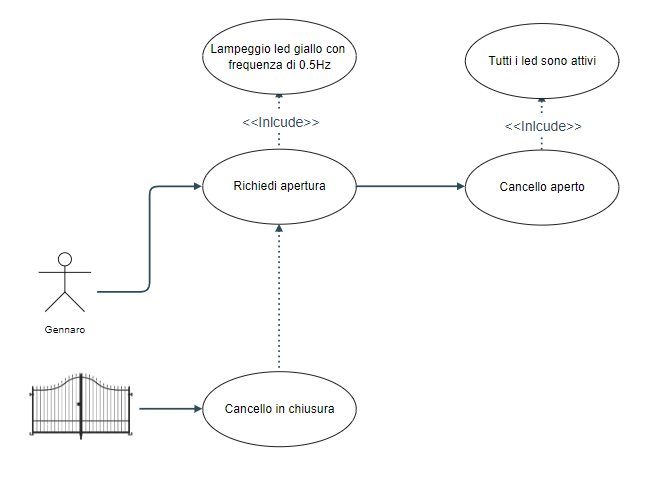
\includegraphics[width=0.6\textwidth,height=5.2cm]{use_case_us1.PNG}
        \caption{USE CASE user story 1.}
        \label{fig:use_case_us1}
    \end{figure}
    
\subsection{Chiusura cancello [US2]}
Questo caso d'uso, che modella US2, ha come attori l'utente e il cancello e descrive la situazione in cui l'utente desidera chiudere il cancello, sia quando è aperto che quando si sta aprendo. L'apertura viene segnalata tramite l'illuminazione del relativo LED giallo. Il cancello chiuso vine segnalato dagli appositi LED verde, giallo e rosso tutti spenti.
\begin{figure}[H]
    \centering
    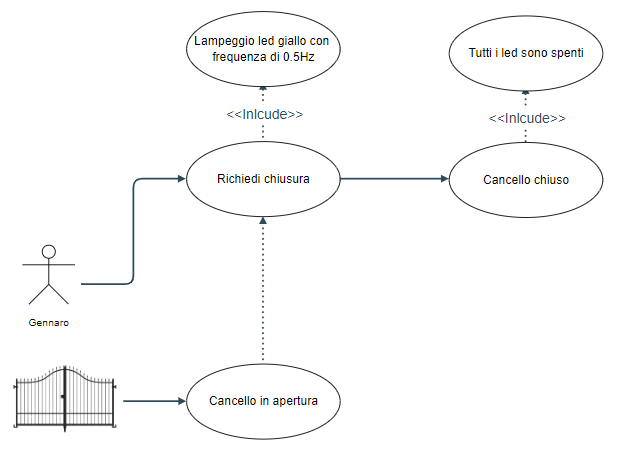
\includegraphics[width=0.6\textwidth,height=5.2cm]{use_case_us2.PNG}
    \caption{USE CASE user story 2.}
    \label{fig:use_case_us2}
\end{figure}

\subsection{Regolazione tempo di chiusura [US3]}
Questo caso d'uso, che modella US3, ha come attore l'utente, che tramite la pressione di un pulsante, può aumentare ciclicamente di 10 secondi, da un minimo di 10 a un massimo di 120, il tempo di chiusura automatica del cancello.
    \begin{figure}[H]
        \centering
        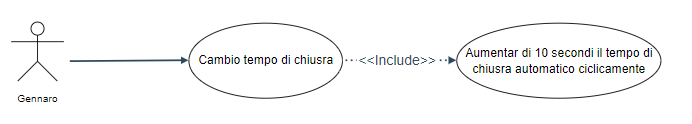
\includegraphics[width=0.8\textwidth]{use_case_us3.PNG}
        \caption{USE CASE user story 3.}
        \label{fig:use_case_us3}
    \end{figure}
\subsection{Regolazione tempo di lavoro [US4]}
Questo caso d'uso, che modella US4, ha come attore l'utente, che tramite la pressione di un pulsante, può aumentare ciclicamente di 10 secondi, da un minimo di 10 a un massimo di 120, il tempo di lavoro del cancello.
    \begin{figure}[H]
        \centering
        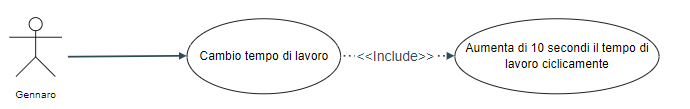
\includegraphics[width=0.8\textwidth]{use_case_us4.PNG}
        \caption{USE CASE user story 4.}
        \label{fig:use_case_us4}
    \end{figure}
\subsection{Riapertura ostacolo [US5]}
Questo caso d'uso, che modella US5, ha come attori l'utente e il cancello. Descrive la situazione in cui il cancello si sta chiudendo e successivamente arriva un ostacolo davanti a esso (sotto il sensore P1), causando la riapertura del cancello.
    \begin{figure}[H]
        \centering
        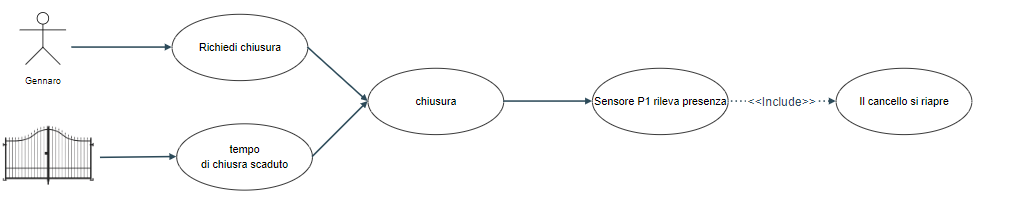
\includegraphics[width=0.8\textwidth]{use_case_us5.PNG}
        \caption{USE CASE user story 5.}
        \label{fig:use_case_us5}
    \end{figure}
\newpage
\subsection{Ignora comando ostacolo [US6]}
Questo caso d'uso, che modella US6, ha come attore l'utente che richiede l'apertura. Tuttavia, se è presente un ostacolo davanti al sensore P1, il comando viene ignorato. Tale situazione viene segnalata dall'attivazione del relativo LED verde per 30 secondi.
    \begin{figure}[h]
        \centering
        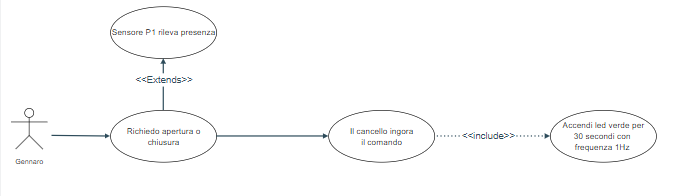
\includegraphics[width=0.8\textwidth]{use_case_us6.PNG}
        \caption{USE CASE user story 6.}
        \label{fig:use_case_us6}
    \end{figure}

\subsection{Stato errore sensore P2 [US7]}
Questo caso d'uso, che modella US7, ha come attore il cancello, che entra in uno stato di allarme se non si chiude entro il tempo di lavoro più 10 secondi. La situazione di allarme viene segnalata dall'attivazione del relativo LED rosso.
\begin{figure}[H]
    \centering
    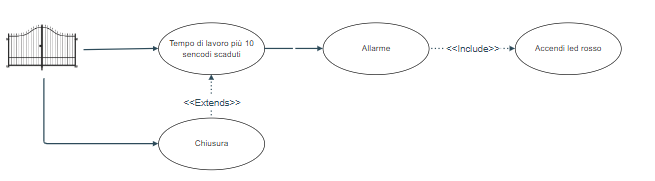
\includegraphics[width=0.8\textwidth]{use_case_us7.PNG}
    \caption{USE CASE user stories 7.}
    \label{fig:use_case_us7}
\end{figure}
\subsection{Chiusura automatica è [US8]}
Questo caso d'uso, che modella US8, ha come attore il cancello, il quale chiude automaticamente il cancello dopo che è trascorso il tempo di lavoro.
    \begin{figure}[H]
        \centering
        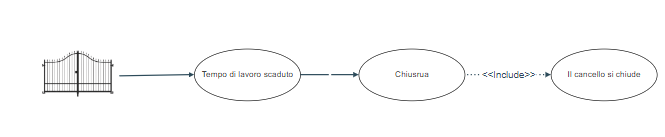
\includegraphics[width=0.8\textwidth]{use_case_us8.PNG}
        \caption{USE CASE user stories 8.}
        \label{fig:use_case_us8}
    \end{figure}
\subsection{Chiusura automatica [US9]}
Questo caso d'uso, che modella US9, ha come attore il cancello. Quando viene acceso, entra nella fase di chiusura se il sensore P2 non è attivo, ovvero se il cancello è aperto e il sensore P1 non è attivo.
    \begin{figure}[H]
        \centering
        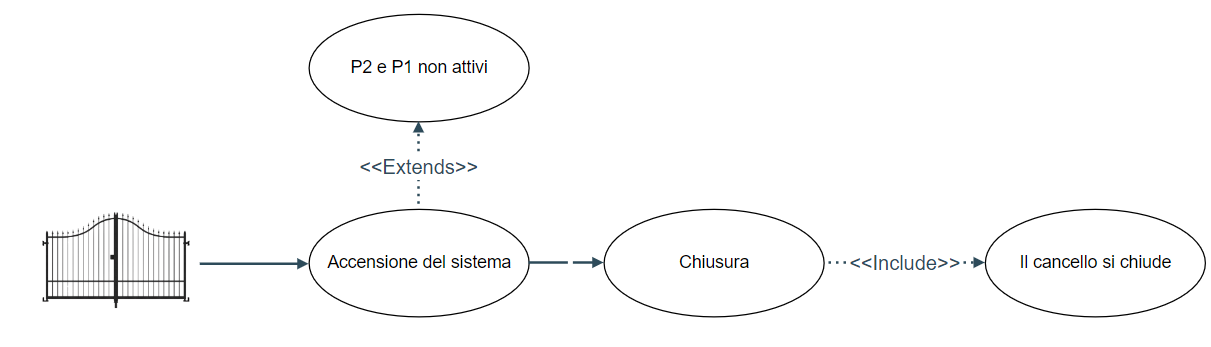
\includegraphics[width=0.8\textwidth]{use_case_us9.PNG}
        \caption{USE CASE user stories 9.}
        \label{fig:use_case_us9}
    \end{figure}
\newpage
\begin{landscape}
\subsection{Use Case Diagram generale}
In questo diagramma dei casi d'uso generale possiamo vedere tutte le azioni che l'utente può compiere per interagire con il sistema, così come le azioni automatiche del sistema che si attivano anche senza la presenza dell'utente.
\begin{figure}[H] % 'h' significa "here", posiziona l'immagine qui
    \centering % Centra l'immagine
    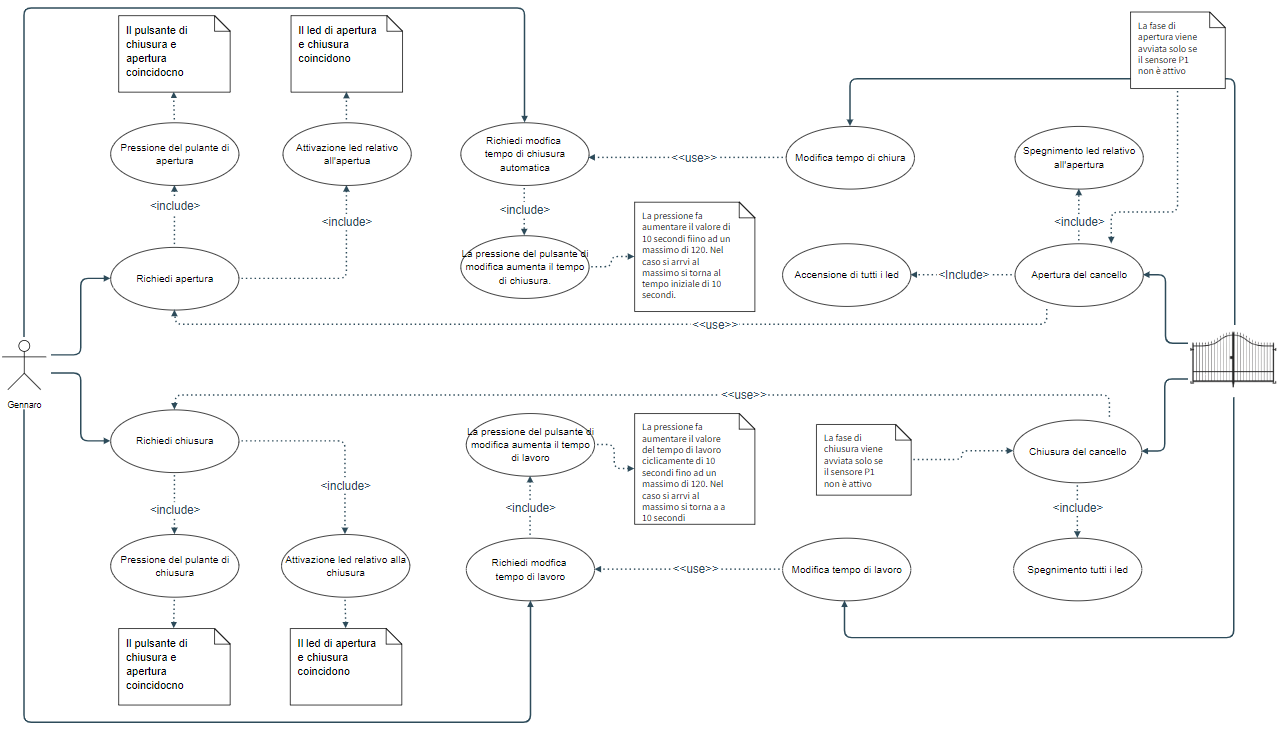
\includegraphics[width=1.35\textwidth]{usa_case_diagram.PNG} % Inserisce l'immagine con una larghezza del 50% del testo
    \caption{Use case diagram} % Aggiunge una didascalia
    \label{fig:General Use Case Diagram} % Aggiunge un'etichetta per riferimenti incrociati
\end{figure}
\end{landscape}

\newpage
\section{Activity Diagrams}
Continuiamo con la presentazione di alcuni diagrammi di attività, strumenti visivi che illustrano il flusso di controllo e le operazioni eseguite dal sistema. Questi diagrammi sono fondamentali per comprendere i vari processi interni del sistema e le loro interconnessioni.
La modellazione degli activity diagrams è stata realizzata su diversi scenari, ognuno dei quali rappresenta un tipico funzionamento del sistema in base alle varie situazioni possibili. A seguire, saranno presentate le descrizioni di ciascuno scenario insieme ai relativi diagrammi di attività.

\subsection{Scenario 1}
Viene presentato in Figura ... il flusso di azioni che l’utente compie per l’apertura del cancello elettrico, dalla fase iniziale della pressione del pulsante, all’apertura completa e infine alla chiusura:

\begin{enumerate}
    \item Per avviare il processo di apertura, l’utente preme il pulsante B1.
    \item Una volta premuto il pulsante, il cancello inizia la fase di apertura e il LED giallo lampeggia.
    \item Il cancello continua ad aprirsi fino al completamento del tempo di lavoro impostato.
    \item Una volta che il cancello è completamente aperto, tutti i LED si accendono.
    \item L'utente può premere di nuovo il pulsante B1 per chiudere il cancello o attendere che passi il tempo di chiusura precedentemente impostato.
\end{enumerate}

\begin{figure}[H]
    \centering
    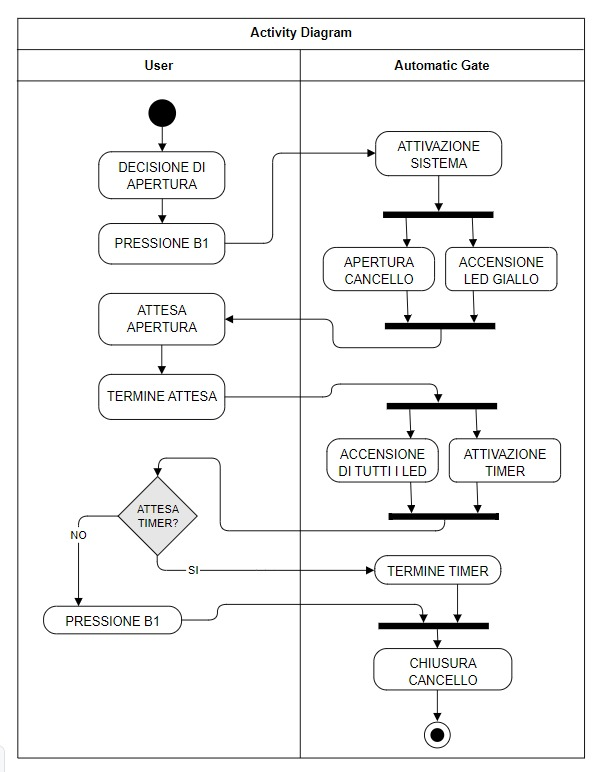
\includegraphics[width = 0.7 \textwidth ]{Scenario_1.jpg}
    \caption{Scenario 1: Apertura e Chiusura Cancello.}
    
\end{figure}

\subsection{Scenario 2}
Questo scenario, presentato in Figura ..., descrive le azioni per l’apertura del cancello elettrico, dalla fase iniziale della pressione del pulsante, all’apertura completa e infine alla chiusura, considerando che venga rilevato un ostacolo durante queste fasi:
\begin{enumerate}
    \item Per avviare il processo di apertura, l’utente preme il pulsante B1.
    \item Una volta premuto il pulsante, il cancello inizia la fase di apertura e il LED giallo lampeggia se non è presente un ostacolo davanti al sensore P1, altrimenti il comando deve essere ripetuto.
    \item Il cancello continua ad aprirsi fino al completamento del tempo di lavoro.
    \item Una volta che il cancello è completamente aperto, tutti i LED si accendono.
    \item L'utente può premere di nuovo il pulsante B1 per chiudere il cancello o attendere che passi il tempo di chiusura precedentemente impostato.
    \item Il cancello entra in fase di chiusura.
    \item Se il sensore P1 rileva la presenza di un ostacolo durante la chiusura, il cancello interrompe la chiusura e inizia la fase di apertura.
    \item L’utente può rimuovere l’ostacolo e il cancello può essere nuovamente chiuso premendo il pulsante B1 o attendendo il tempo di chiusura automatica.
\end{enumerate}

\begin{figure}[h]
    \centering
    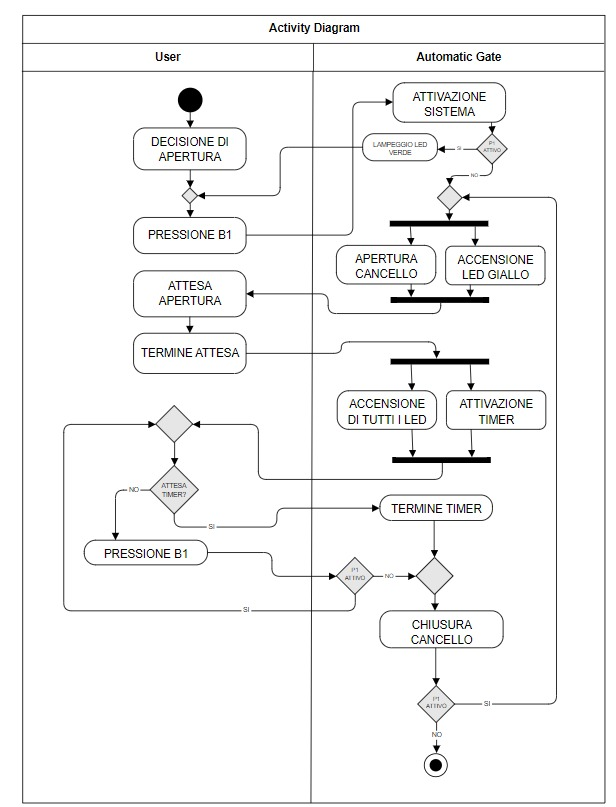
\includegraphics[width = 0.7 \textwidth ]{Scenario_2.jpg}
    \caption{Scenario 2: Apertura e Chiusura con Ostacoli.}
    
\end{figure}

\subsection{Scenario 3}
Lo scenario, presentato in Figura ..., descrive le attività quando il cancello entra in uno stato di errore se non si chiude entro il tempo di lavoro previsto. Nel seguito verrà presentato il flusso di azioni associato allo scenario corrente:

\begin{enumerate}
    \item Il sistema viene attivato.
    \item L'utente preme il pulsante di apertura (B1).
    \item Il cancello inizia la fase di apertura.
    \item La fase di apertura termina.
    \item Il cancello passa alla fase di chiusura.
    \item Il tempo di lavoro impostato viene superato senza che il sensore P2 rilevi la chiusura completa.
    \item Il LED rosso si accende per notificare lo stato di errore.
    \item L’utente deve intervenire per risolvere il problema e riportare il sistema in uno stato operativo normale.
\end{enumerate}

\begin{figure}[h]
    \centering
    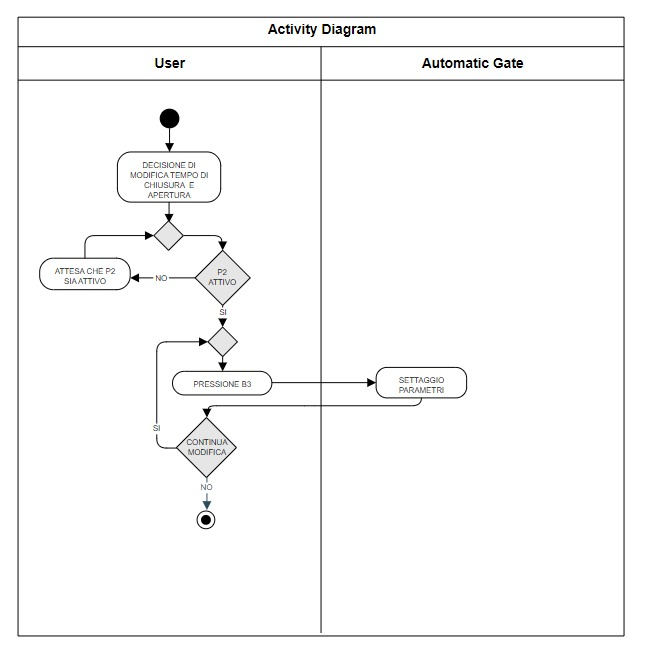
\includegraphics[width = 0.7 \textwidth]{Scenario_3.jpg}
    \caption{Scenario 3: Stato di Errore.}
    
\end{figure}

\newpage
\subsection{Scenario 4}
Questo scenario, presentato in Figura ..., descrive le azioni che l’utente compie per regolare il tempo di apertura e chiusura (tempo di lavoro) del cancello elettrico utilizzando il pulsante B3:

\begin{enumerate}
    \item L’utente decide di regolare il tempo di apertura e chiusura (tempo di lavoro).
    \item Per impostare il tempo di apertura e chiusura, l’utente preme ripetutamente il pulsante B3.
    \item Ogni pressione del pulsante B3 aumenta il tempo di lavoro di 10 secondi.
    \item Una volta impostato il tempo desiderato, l’utente termina l’operazione e il cancello utilizzerà il tempo impostato per le operazioni di apertura e chiusura.
\end{enumerate}

\begin{figure}[h]
    \centering
    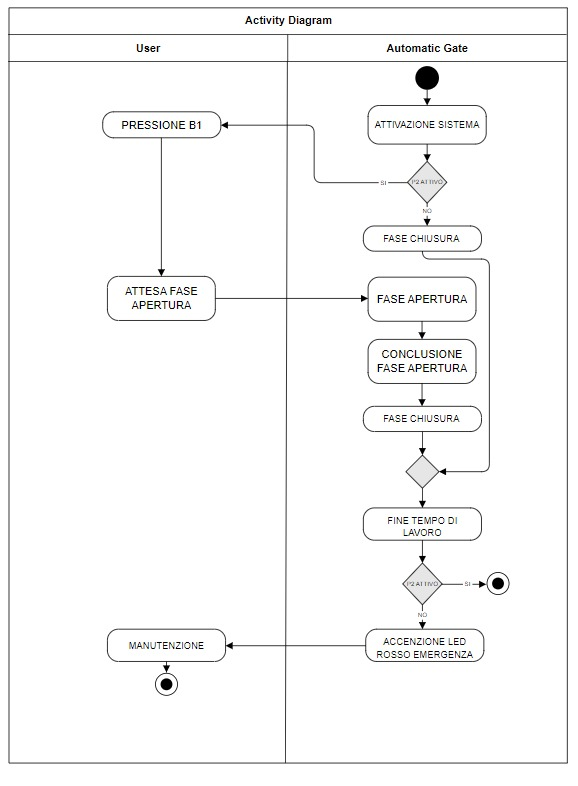
\includegraphics[width = 0.7 \textwidth]{Scenario_4.jpg}
    \caption{Scenario 1: Regolazione del Tempo di Lavoro}
    
\end{figure}

\newpage

\section{State diagram}
Nell'ultima parte di questa relazione si illustra lo State Diagram che ha lo scopo di descrivere quali sono i vari stati in cui il sistema si può trovare. Lo state diagram è utile per chiarire il comportamento del cancello rispetto agli eventi interni ed esterni che possono essere interpretati diversamente a seconda dello stato in cui si trova.
I principali stati del cancello automatico descritto nei capitoli precedenti sono:
\begin{itemize}
    \item{\textbf{CLOSING,}} è lo stato iniziale del sistema.
    \item{\textbf{CLOSED,}} è lo stato che si raggiunge quando la seconda fotocellula (P2) è occupata durante il quale tutti i led sono spenti. Quando il sistema si trova in questo stato è possibile impostare il tempo di lavoro e quello di chiusura da 10 a 120 secondi.
    \item {\textbf{OPEN\_DUR\_SETTING,}} questo stato imposta il tempo che il cancello deve rimanere nello stato aperto se non si è richiesta la chiusura.
    \item {\textbf{WORK\_DUR\_SETTING}} questo stato imposta il tempo che impiega il cancello ad aprirsi.
    \item{\textbf{OPENING,}} è lo stato di apertura del cancello durante il quale in led giallo lampeggia.
    \item{\textbf{OPEN,}} è lo stato in cui il cancello è aperto e tutti i led sono accesi.
\end{itemize}

In parallelo a questi ci sono gli stati \textbf{B1}, \textbf{B2} e 
\textbf{B3}, che "ascoltano" i fronti di salita provenienti dai rispettivi bottoni.
Si ricorda che B1 permette di richiedere l'apertura o la chiusura, B2 imposta il tempo di chiusura e, infine, B3 imposta il tempo di lavoro.\\

Gli altri stati che non sono elencati sopra sono importanti in quanto gestiscono situazioni di errore ed emergenza. Sono elencati qui:

\begin{itemize}
    \item{\textbf{EMERGENCY\_P1\_CLOSED,}} è uno stato che viene raggiunto nel caso in sui si richiede l'apertura del cancello, ma il sensore P1 è impegnato. l led verde lampeggia per 30 sec.
    \item{\textbf{EMERGENCY\_P1\_OPEN,}} è corrispettivo dello stato precedente nel caso in cui si richiede la chiusura del cancello mentre P1 è impegnato. Il led verde lampeggia per 30 sec.
    \item{\textbf{EMERGENCY,}} viene raggiunto nel caso in cui P2 non viene impegnato entro il tempo di lavoro. Il sistema esce da questo stato dopo 10 secondi oppure quando viene impegnato P2.
    \item{\textbf{EMERGENCY\_LED}}, viene raggiunto se lo stato \textbf{EMERGENCY} permane per più di 10 secondi. In questo stato viene attivato il led rosso.
\end{itemize}

Di seguito sono illustrati il diagramma di stato di un pulsante che vale anche per gli altri, e successivamente è illustrato lo schema generico del cancello automatico. E' stata inserita un'immagine che rappresenta anche lo stato \textbf{CLOSED} in particolare. Questo stato comprende che gli stati per aumentare il tempo di lavoro e quello di chiusura.
\newpage
\begin{landscape}
\begin{figure}[h] % 'h' significa "here", posiziona l'immagine qui
    \centering % Centra l'immagine
    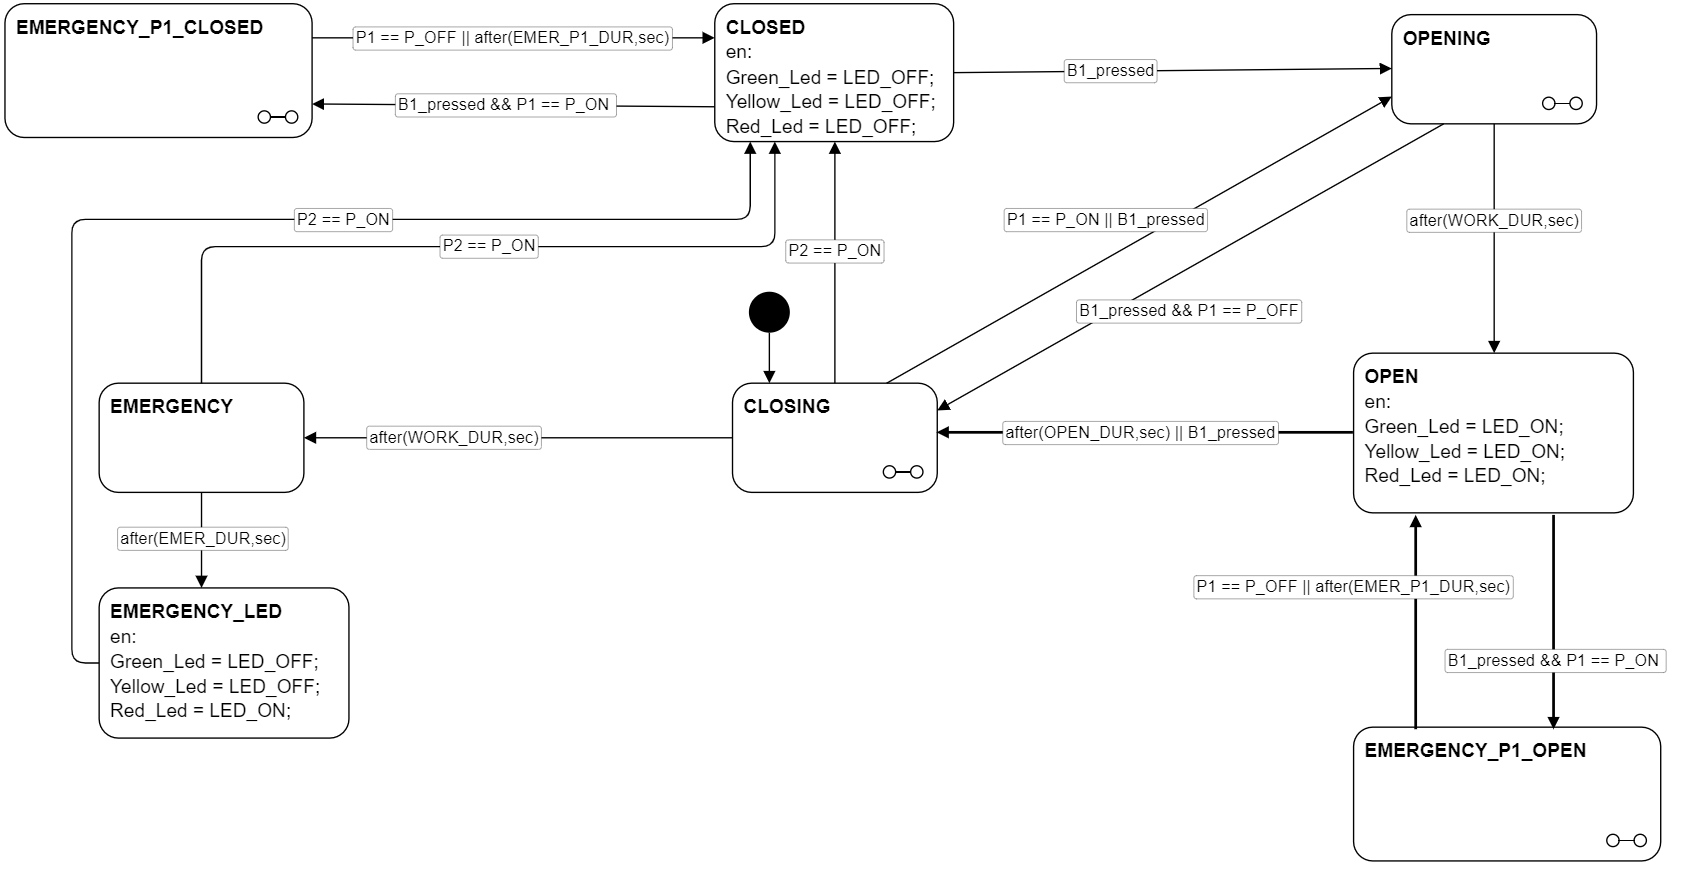
\includegraphics[width=1.5\textwidth]{state_diagram0.png} % Inserisce l'immagine con una larghezza del 50% del testo
    \caption{General State Diagram} % Aggiunge una didascali
    \label{fig:General State Diagram} % Aggiunge un'etichetta per riferimenti incrociati
\end{figure}
\end{landscape}

\begin{figure}[h] % 'h' significa "here", posiziona l'immagine qui
    \centering % Centra l'immagine
    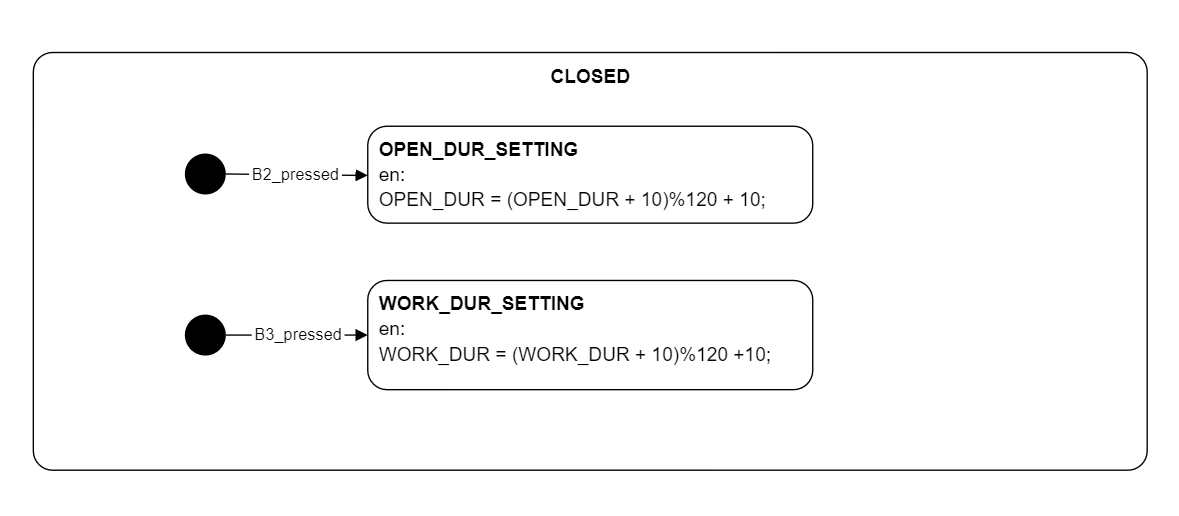
\includegraphics[width=1\textwidth]{state_diagram1.png} % Inserisce l'immagine con una larghezza del 50% del testo
    \caption{CLOSED State} % Aggiunge una didascalia
    \label{fig:CLOSED State} % Aggiunge un'etichetta per riferimenti incrociati
\end{figure}

\begin{figure}[h] % 'h' significa "here", posiziona l'immagine qui
    \centering % Centra l'immagine
    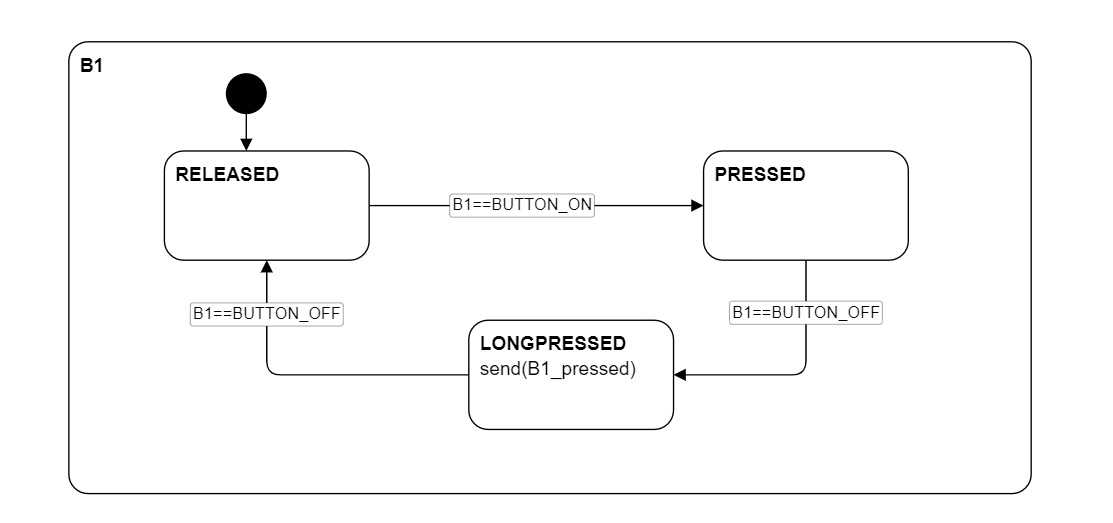
\includegraphics[width=1\textwidth]{state_diagram2.png} % Inserisce l'immagine con una larghezza del 50% del testo
    \caption{Button State} % Aggiunge una didascalia
    \label{fig:Button State} % Aggiunge un'etichetta per riferimenti incrociati
\end{figure}
\newpage
\addcontentsline{toc}{section}{Elenco delle figure}
\listoffigures
\end{document}
